\chapter{Porte Logiche e Algebra di Boole}

I circuiti digitali vengono realizzati utilizzando componenti chiamati \textbf{porte logiche}. Sono realizzate con componenti fisici come transistor e resistenze, ma nella progettazione dei circuiti digitali le porte logiche vengono schematizzate con i simboli riportati nella Figura 3.1 per semplificare la progettazione \textbf{astraendo} il livello di complessità della circuiteria analogica.
Solamente con la porta NAND si possono realizzare tutte le altre porte (NAND è funzionalmente completo), ma le porte in generale si costruiscono singolarmente con componenti appositi. Esse implementano la \textbf{logica booleana} che conseguentemente permette di realizzare operazioni di \textbf{aritmetica binaria} per costruire unità di calcolo in componenti elettronici e processori.

\begin{wrapfigure}{r}{0.6\textwidth}
	\begin{center}
		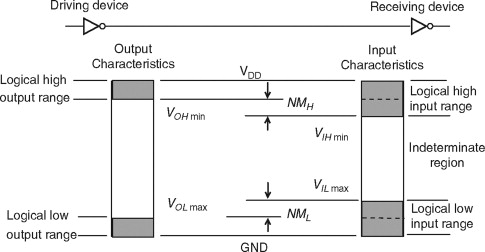
\includegraphics[width=0.58\textwidth]{noisemargin}
	\end{center}
	\caption{Margine di rumore nei circuiti digitali}	
\end{wrapfigure}


I componenti elettronici molto piccoli sono sensibili al \textbf{rumore}, per ovviare al problema i valori discreti (0 e 1) nei circuiti digitali non seguono un cambiamento istantaneo di differenza di potenziale (voltaggio), ma ammettono un margine per ridurre i problemi causati dal rumore.


I componenti (transistor) con cui si costruiscono porte logiche e circuiti sono realizzati con materiali semiconduttori, che possono essere di diversi tipi. Vedremo il tipo NMOS. Un transistor è composto da materiali come gallio e silicio.

\begin{wrapfigure}{r}{0.7\textwidth}
	\begin{center}
		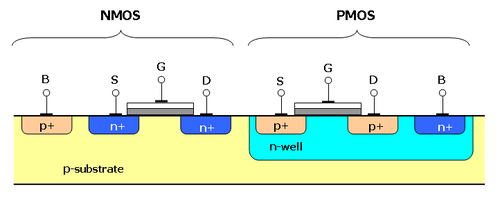
\includegraphics[width=0.68\textwidth]{cmos}
	\end{center}
	\caption{Transistor NMOS}
\end{wrapfigure}


\begin{figure}
	\centering
	\caption{Tabella delle porte logiche comuni}
	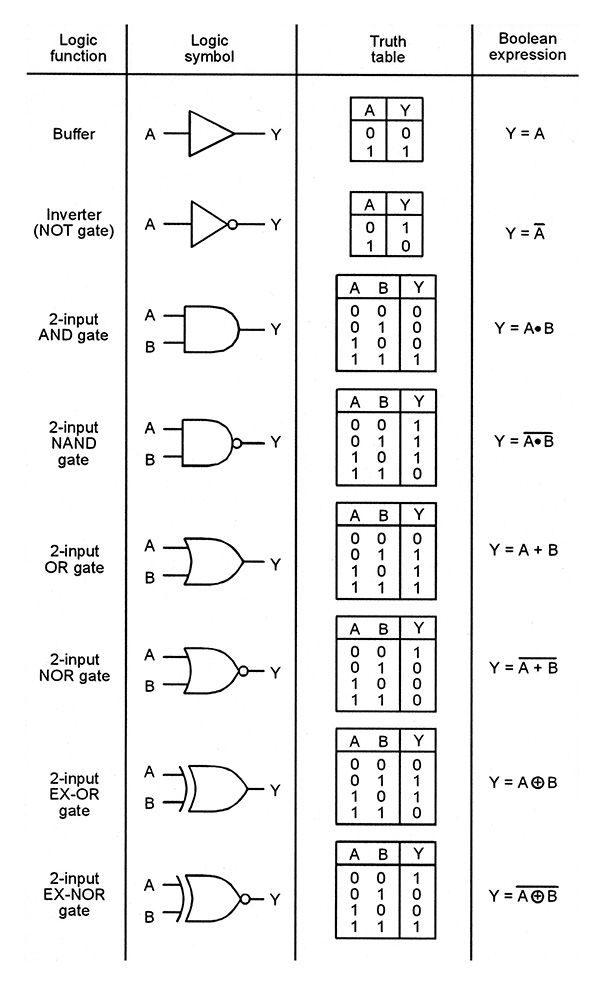
\includegraphics[width=\textwidth,height=\textheight]{logicgates}
\end{figure}

\begin{figure}
	\centering
	\caption{Porta NOT con transistor PMOS e NMOS}
	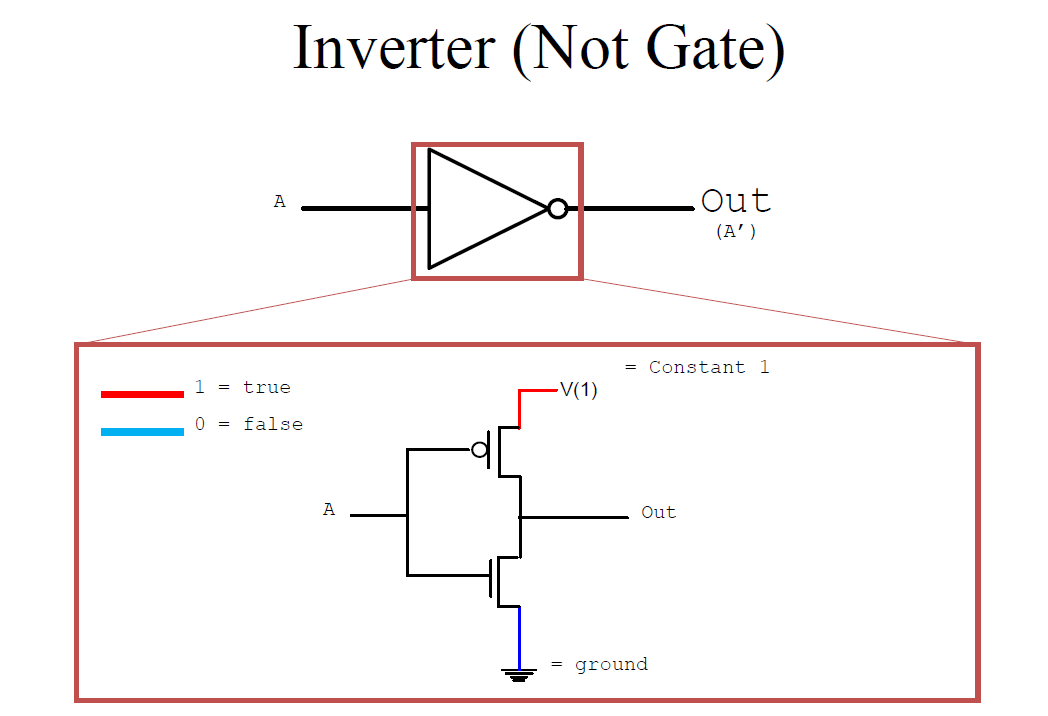
\includegraphics[width=\textwidth]{notgatetransistor}
\end{figure}

\begin{figure}
	\centering
	\caption{Transistor NMOS e PMOS}
	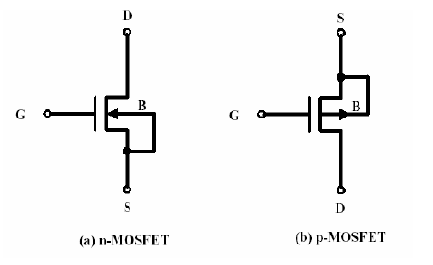
\includegraphics[width=0.6\textwidth]{NMOS-and-PMOS}
\end{figure}

\clearpage

\section{Algebra di Boole}


\begin{figure}[H]
	\centering
	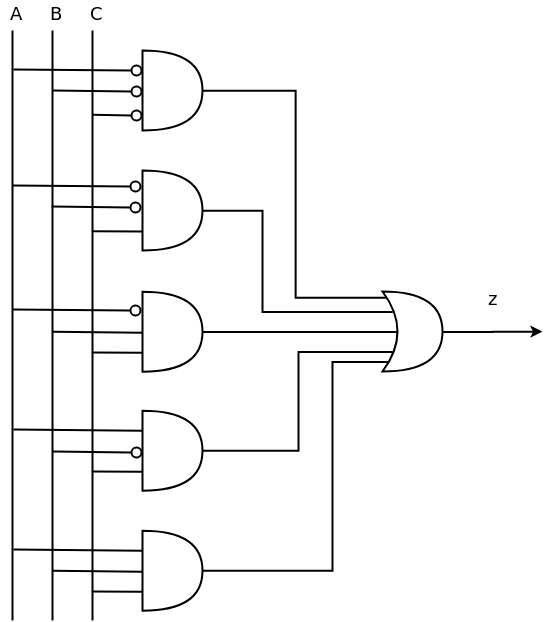
\includegraphics[width=0.48\textwidth]{sommadiprodotti-gate}
	\caption{Conversione di $ z $ da formula booleana a circuito logico}
\end{figure}

\begin{table}[H]
	\centering
	\caption{Notazione usata per l'Algebra di Boole}
	\label{tab:notazione-booleana}
	\begin{tabular}{|l|l|l|}
		\hline
		Funzione & Notazione Usata & Notazione Logica \\ 
		NOT(A)   & $\overbar{A}$   & $\lnot A$        \\ 
		AND(A,B) & $A \cdot B$     & $A \land B$      \\ 
		OR(A,B)  & $A + B$         & $A \lor B$       \\ \hline
	\end{tabular}
\end{table}

Prendiamo ad esempio un espressione booleana in forma canonica in \textbf{somma di prodotti} è:
\[ z = \overbar{A}\overbar{B}\overbar{C} + \overbar{A}\overbar{B}C + \overbar{A}BC + A\overbar{B}C + ABC \]


\begin{table}[H]
	\centering
	\caption{Tabella di verità di $ z $}
	\label{tab:z-truth}
	\begin{tabular}{|l|l|l|l|}
		\hline
		A & B & C & z \\ \hline
		0                       & 0                      & 0 & 1 \\  
		0                       & 0                      & 1 & 1 \\ 
		0                       & 1                      & 0 & 0 \\ 
		0                       & 1                      & 1 & 1 \\ 
		1                       & 0                      & 0 & 0 \\ 
		1                       & 0                      & 1 & 1 \\  
		1                       & 1                      & 0 & 0 \\ 
		1                       & 1                      & 1 & 1 \\ \hline
	\end{tabular}
\end{table}




$ z $ si può anche esprimere come prodotto di somme: $ z = (A+\overbar{B}+C)(\overbar{A}BC)(\overbar{A}\overbar{B}C) $


\section{Teoremi dell'Algebra Booleana}
Breve ripasso dei teoremi della Logica Booleana.
\paragraph{Elemento Identità di prodotto e somma}
\[ A \cdot 1 = A \iff A \land T \equiv A\]
\[ A + 0 = 0 \iff A \lor F \equiv A\]
\paragraph{Elemento assorbente}
\[ A \cdot 0 = 0 \iff A \land F \equiv F \]
\[ A + 1 = 1 \iff A \lor T \equiv T \]
\paragraph{Idempotenza}
\[ A \cdot A = A \iff A \land A \equiv A \]
\[ A + A = A \iff A \lor A \equiv A \]
\paragraph{Complemento}
\[ A \cdot \overbar{A} = 0 \iff A \land \lnot A \equiv F \]
\[ A + \overbar{A} = 1 \iff A \lor \lnot A \equiv T \]
\paragraph{Commutatività}
\[ A + B = B + A \]
\[ A \cdot B = B \cdot A \]
\paragraph{Associatività}
\[ (A \cdot B) \cdot C = A \cdot (B \cdot C) \]
\[ (A + B) + C = A + (B + C) \]
\paragraph{Distributività}
\[ (A \cdot B) + C = (A+C) \cdot (B+C) \]
\[ (A+B) \cdot C = AC + BC \]
\paragraph{DeMorgan}
\[ \overbar{(A + B)} = \overbar{A} \cdot \overbar{B} \iff \lnot(A \lor B )\equiv \lnot A \land \lnot B \]
\[ \overbar{(A \cdot B)} = \overbar{A} + \overbar{B} \iff \lnot(A \land B )\equiv \lnot A \lor \lnot B \]

\paragraph{Esempio}
Semplifichiamo la formula booleana $ z = \overbar{A}\overbar{B}\overbar{C} + \overbar{A}\overbar{B}C + \overbar{A}BC + A\overbar{B}C + ABC $

\begin{align}
\begin{cases}
\overbar{A}\overbar{B}\overbar{C} + \overbar{A}\overbar{B}C \equiv \overbar{A}\overbar{B}(\overbar{C}+C) \equiv \overbar{A}\overbar{B} \\ 
A\overbar{B}C + ABC \equiv AC(\overbar{B}+B) \equiv AC
\end{cases} \\
\implies z = \overbar{A}\overbar{B} + \overbar{A}BC + AC
\end{align}

Le leggi della logica Booleana ci permettono di semplificare molto i componenti realizzati con porte logiche.

\section{Mappe di Karnaugh}

Una mappa di Karnaugh o K-Map è un metodo di semplificare un espressione booleana. I valori sono trasferiti da una tabella di verità ad una mappa bidimensionale:

Approfondisci su \href{https://en.wikipedia.org/wiki/Karnaugh_map}{Wikipedia}

Prendiamo una formula a quattro variabili $ f(A,B,C,D) $, una mappa di Karnaugh può essere:
\begin{table}[H]
	\centering
	\caption{Tabella di verità della mappa di Karnaugh di $f$}
	\label{tab:karnaugh}
	\begin{tabular}{lllll}
		AB\textbackslash{}CD    & 00                     & 01                     & 11                     & 10                     \\ \cline{2-5} 
		\multicolumn{1}{l|}{00} & \multicolumn{1}{l|}{1} & \multicolumn{1}{l|}{1} & \multicolumn{1}{l|}{1} & \multicolumn{1}{l|}{1} \\ \cline{2-5} 
		\multicolumn{1}{l|}{01} & \multicolumn{1}{l|}{1} & \multicolumn{1}{l|}{1} & \multicolumn{1}{l|}{0} & \multicolumn{1}{l|}{0} \\ \cline{2-5} 
		\multicolumn{1}{l|}{11} & \multicolumn{1}{l|}{0} & \multicolumn{1}{l|}{1} & \multicolumn{1}{l|}{0} & \multicolumn{1}{l|}{0} \\ \cline{2-5} 
		\multicolumn{1}{l|}{10} & \multicolumn{1}{l|}{0} & \multicolumn{1}{l|}{0} & \multicolumn{1}{l|}{1} & \multicolumn{1}{l|}{1} \\ \cline{2-5} 
	\end{tabular}
\end{table}

Facciamo ad esempio la mappa di Karnaugh di $ z = f(A,B,C) $ vista nella sezione precedente:

\begin{table}[H]
	\centering
	\caption{Tabella di verità della mappa di Karnaugh di $z$}
	\label{tab:karnaugh}
	\begin{tabular}{lllll}
		A\textbackslash{}BC    & 00                     & 01                     & 11                     & 10                     \\ \cline{2-5} 
		\multicolumn{1}{l|}{0} & \multicolumn{1}{l|}{1} & \multicolumn{1}{l|}{1} & \multicolumn{1}{l|}{1} & \multicolumn{1}{l|}{0} \\ \cline{2-5} 
		\multicolumn{1}{l|}{1} & \multicolumn{1}{l|}{0} & \multicolumn{1}{l|}{1} & \multicolumn{1}{l|}{1} & \multicolumn{1}{l|}{0} \\ \cline{2-5} 
	\end{tabular}
\end{table}

Possiamo riconoscere un'implicante nella seconda e terza colonna che corrisponde esattamente a C. Osserviamo un'altra implicante nella prima riga, prima e seconda colonna che corrisponde esattamente a $ \overbar{A}\overbar{B} $. Possiamo poi sommare le implicanti per ottenere una formula equivalente a quella di partenza, ciò implica che $ z =  \overbar{A}\overbar{B} + C $


\subsection{Circuito con più output}
Se abbiamo una tabella di verità di un circuito con $ n $ input e $ 2^n $ righe, con più output $ z_1, \dots, z_k $, gli output si suddividono in $ k $ tabelle con un solo output ($ z_k $) e $ 2^n $ righe di input.